%----------------------------------------------------------------------------------------
%	PACKAGES AND OTHER DOCUMENT CONFIGURATIONS
%----------------------------------------------------------------------------------------

\documentclass{article}

\usepackage{fancyhdr} % Required for custom headers
\usepackage{lastpage} % Required to determine the last page for the footer
\usepackage{extramarks} % Required for headers and footers
\usepackage{graphicx} % Required to insert images
\usepackage{amsmath, amssymb} % Required for Maths
\usepackage{mathtools} % Required for Maths
\usepackage{enumerate}
\usepackage{mathtools}
\usepackage{textcomp}
\usepackage{gensymb}
\usepackage{siunitx}
\usepackage{empheq}
\usepackage{ulem}
\usepackage{amssymb}

% Margins
\topmargin=-0.45in
\evensidemargin=0in
\oddsidemargin=0in
\textwidth=6.5in
\textheight=9.0in
\headsep=0.25in 

\linespread{1.1} % Line spacing

% Set up the header and footer
\pagestyle{fancy}
\lhead{\hmwkAuthorName} % Top left header
\chead{\hmwkClass\ (\hmwkClassInstructor\ \hmwkClassTime): \hmwkTitle} % Top center header
\rhead{\firstxmark} % Top right header
\lfoot{\lastxmark} % Bottom left footer
\cfoot{} % Bottom center footer
\rfoot{Page\ \thepage\ of\ \pageref{LastPage}} % Bottom right footer
\renewcommand\headrulewidth{0.4pt} % Size of the header rule
\renewcommand\footrulewidth{0.4pt} % Size of the footer rule

\setlength\parindent{0pt} % Removes all indentation from paragraphs

%----------------------------------------------------------------------------------------
%	DOCUMENT STRUCTURE COMMANDS
%	Skip this unless you know what you're doing
%----------------------------------------------------------------------------------------

% Header and footer for when a page split occurs within a problem environment
\newcommand{\enterProblemHeader}[1]{
\nobreak\extramarks{#1}{#1 continued on next page\ldots}\nobreak
\nobreak\extramarks{#1 (continued)}{#1 continued on next page\ldots}\nobreak
}

% Header and footer for when a page split occurs between problem environments
\newcommand{\exitProblemHeader}[1]{
\nobreak\extramarks{#1 (continued)}{#1 continued on next page\ldots}\nobreak
\nobreak\extramarks{#1}{}\nobreak
}

\setcounter{secnumdepth}{0} % Removes default section numbers
\newcounter{homeworkProblemCounter} % Creates a counter to keep track of the number of problems

\newcommand{\homeworkProblemName}{}
\newenvironment{homeworkProblem}[1][Problem \arabic{homeworkProblemCounter}]{ % Makes a new environment called homeworkProblem which takes 1 argument (custom name) but the default is "Problem #"
\stepcounter{homeworkProblemCounter} % Increase counter for number of problems
\renewcommand{\homeworkProblemName}{#1} % Assign \homeworkProblemName the name of the problem
\section{\homeworkProblemName} % Make a section in the document with the custom problem count
\enterProblemHeader{\homeworkProblemName} % Header and footer within the environment
}{
\exitProblemHeader{\homeworkProblemName} % Header and footer after the environment
}

\newcommand{\problemAnswer}[1]{ % Defines the problem answer command with the content as the only argument
\noindent\framebox[\columnwidth][c]{\begin{minipage}{0.98\columnwidth}#1\end{minipage}} % Makes the box around the problem answer and puts the content inside
}

\newcommand{\homeworkSectionName}{}
\newenvironment{homeworkSection}[1]{ % New environment for sections within homework problems, takes 1 argument - the name of the section
\renewcommand{\homeworkSectionName}{#1} % Assign \homeworkSectionName to the name of the section from the environment argument
\subsection{\homeworkSectionName} % Make a subsection with the custom name of the subsection
\enterProblemHeader{\homeworkProblemName\ [\homeworkSectionName]} % Header and footer within the environment
}{
\enterProblemHeader{\homeworkProblemName} % Header and footer after the environment
}

%----------------------------------------------------------------------------------------
%	NAME AND CLASS SECTION
%----------------------------------------------------------------------------------------

\newcommand{\hmwkTitle}{Exam\ \#1} % Assignment title
\newcommand{\hmwkDueDate}{Sunday,\ November\ 1,\ 2015} % Due date
\newcommand{\hmwkClass}{ENPM 808M} % Course/class
\newcommand{\hmwkClassTime}{4:00 PM} % Class/lecture time
\newcommand{\hmwkClassInstructor}{Dr. William Levine} % Teacher/lecturer
\newcommand{\hmwkAuthorName}{Kanishka Ganguly} % Your name

%----------------------------------------------------------------------------------------
%	TITLE PAGE
%----------------------------------------------------------------------------------------

\title{
\vspace{2in}
\textmd{\textbf{\hmwkClass:\ \hmwkTitle}}\\
\normalsize\vspace{0.1in}\small{Due\ on\ \hmwkDueDate}\\
\vspace{0.1in}\large{\textit{\hmwkClassInstructor\ \hmwkClassTime}}
\vspace{3in}
}

\author{\textbf{\hmwkAuthorName}}
\date{} % Insert date here if you want it to appear below your name

%----------------------------------------------------------------------------------------

\begin{document}

\maketitle

%----------------------------------------------------------------------------------------
%	TABLE OF CONTENTS
%----------------------------------------------------------------------------------------

%\setcounter{tocdepth}{1} % Uncomment this line if you don't want subsections listed in the ToC

\newpage
\tableofcontents
\newpage

%----------------------------------------------------------------------------------------
%	PROBLEM 1
%----------------------------------------------------------------------------------------
\begin{homeworkProblem}
To prove that the following homogenous transformations are correct:
\begin{homeworkSection}{(a)}
\begin{align}
H = 
\begin{bmatrix}
\cos(\theta_1) & 0 & -sin(\theta_1) & -sin(\theta_1)d_3\\
\sin(\theta_1) & 0 & cos(\theta_1) & cos(\theta_1)d_3\\
     0 		   & 1 &       0        & d_1 -d_2\\
     0         & 0 &       0        &          1
\end{bmatrix}
\end{align}

This matrix is a combination of a rotational matrix $H_R$ and a translational matrix $H_{R_d}$ and is of the form
\begin{align}
\begin{bmatrix}
H_R & H_{R_d}\\
0 & 1
\end{bmatrix}
\end{align}

The matrix $H$ can thus be split into the following matrices:
\begin{align}
H_R=
\begin{bmatrix}
\cos(\theta_1) & 0 & -sin(\theta_1) & 0\\
\sin(\theta_1) & 0 & cos(\theta_1) & 0\\
0 & 1 & 0 & 0\\
0 & 0 & 0 & 1
\end{bmatrix}
H_{R_d}=
\begin{bmatrix}
0 & 0 & 0 & -sin(\theta_1)d_3\\
0 & 0 & 0 & cos(\theta_1)d_3\\
0 & 0 & 0 & d_1 - d_2\\
0 & 0 & 0 & 1
\end{bmatrix}
\end{align}

Now, for $H$ to be a valid homogenous transformation matrix, $H_R$ must be a valid rotational matrix.\\
The necessary condition for $H_R$ to be a valid rotation matrix is that $H_R \in SO(3)$. The following conditions must be satisfied:
\begin{itemize}
\item $H_R^{-1} = H_R^T$
\item $det(H_R) = 1$
\item $H_R^{-1} \in SO(3)$
\end{itemize}

Now, consider the condition $det(H_R) = 1$ mentioned above. From calculation of determinant, we get
\begin{align}
det(H_R) = (-1)(sin^2(\theta_1) + cos^2(\theta_1)) = -1
\end{align}
Now, for $H_R$ to be a rotational matrix, $det(H_R) = 1$.\\
However, $det(H_R) = sin^2(\theta_1) + cos^2(\theta_1) \neq 1 $ for any $\theta \in \mathbb{R}$.\\\\
This violates the condition needed for $H_R$ to be a rotational matrix and since $H_R$ is the rotational component of matrix $H$, this implies that \uuline{$H$ is also not a valid homogenous transformation matrix.}
\end{homeworkSection}

\begin{homeworkSection}{(b)}
\begin{align}
T=
\begin{bmatrix}
c_1c_2 & -s_1 & c_1s_2 & c_1s_2d_3 - s_1d_2\\
s_1c_2 & c_1 & s_1s_2 & s_1s_2d_3 + c_1d_2\\
s_2 & 0 & c_2 & c_2d_3\\
0 & 0 & 0 & 1
\end{bmatrix}
\end{align}

The above transformation matrix $T$ can be written in terms of rotational and translational components $T_R$ and $T_{R_d}$ respectively as:
\begin{align}
T = 
\begin{bmatrix}
T_R &  T_{R_d}\\
0 & 1
\end{bmatrix}\\
\implies T_R =
\begin{bmatrix}
c_1c_2 & -s_1 & c_1s_2 & 0\\
s_1c_2 & c_1 & s_1s_2 & 0\\
s_2 & 0 & c_2 & 0\\
0 & 0 & 0 & 1
\end{bmatrix}
\end{align}

For $T$ to be a valid, homogenous transformation matrix, it is necessary for $T_R$ to be a valid rotational matrix. Similar to $(a)$, $T_R$ must satisfy the following conditions for it to be a valid rotation matrix:
\begin{itemize}
\item $T_R^{-1} = T_R^T$
\item $det(T_R) = 1$
\item $T_R^{-1} \in SO(3)$
\end{itemize}

Considering the condition $det(T_R) = 1$, we have from calculation:
\begin{align}
det(T_R) = cos^2(\theta) - sin^2(\theta)
\end{align}
Now, for $T_R$ to be a rotation matrix, $det(T_R) = 1$.\\
But $det(T_R) = cos^2(\theta) - sin^2(\theta) \neq 1$ for any $\theta \in \mathbb{R}$.\\
Thus, the condition is needed for $T_R$ to be a rotation matrix is not satisfied and since $T_R$ is the rotational component of matrix $T$, this implies that \uuline{$T$ is also not a valid homogenous transformation matrix.}
\end{homeworkSection}
\end{homeworkProblem}
\clearpage
%----------------------------------------------------------------------------------------
%	PROBLEM 2
%----------------------------------------------------------------------------------------

\begin{homeworkProblem}
\problemAnswer{ % Answer
\begin{center}
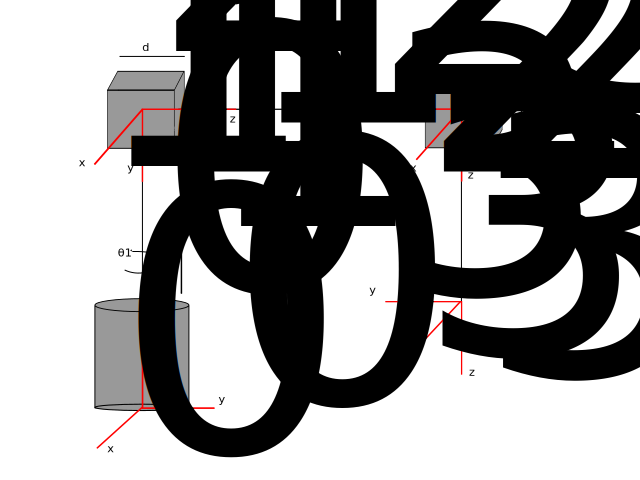
\includegraphics[width=0.75\columnwidth]{img/Q2.png} % Q2_1st Image
\end{center}
}
\vspace{20pt}
Choice of Axes - DH Convention

From given figure, we form DH Parameters as:
\begin{center}
\begin{tabular}{|l|l|l|l|l|{c}r}
\hline
Link ($i$) & $a_i$ & $\alpha_i$ & $d_i$ & $\theta_i$\\
\hline
1 & $0$ & $-90$ & $d_1$ & $\mathbf{\theta_1}$\\
2 & $0$ & $-90$ & $\mathbf{d_2}$ & $0$\\
3 & $0$ & $0$ & $\mathbf{d_3}$ & $0$\\
\hline
\end{tabular}
\end{center}
where \textbf{bold} indicates a variable value.\\

Applying the DH convention, we get the following matrix:
\begin{align}
A_i = 
\begin{bmatrix}
c_{\theta_i} & -s_{\theta_i}c_{\alpha_i} & s_{\theta_i}s_{\alpha_i} & a_ic_{\theta_i}\\
s_{\theta_i} & c_{\theta_i}c_{\alpha_i} & -c_{\theta_i}s_{\alpha_i} & a_is_{\theta_i}\\
0 & s_{\alpha_i} & c_{\alpha_i} & d_i\\
0 & 0 & 0 & 1
\end{bmatrix}
\end{align}
\begin{homeworkSection}{(a)}
We have
\begin{align}
T_1^0 = A_1 = 
\begin{bmatrix}
c_1 & 0 & -s_1 & 0\\
s_1 & 0 & c_1 & 0\\
0 & -1 & 0 & d_1\\
0 & 0 & 0 & 1
\end{bmatrix}\\
T_2^1 = A_2 = 
\begin{bmatrix}
1 & 0 & 0 & 0\\
0 & 0 & 1 & 0\\
0 & -1 & 0 & d_2\\
0 & 0 & 0 & 1
\end{bmatrix}\\
\text{We have:} \quad T_2^0 = T_1^0 \times T_2^1\\
\implies T_2^0 =
\begin{bmatrix}
c_1 & s_1 & 0 & -s_1d_2\\
s_1 & -c_1 & 0 & c_1d_2\\
0 & 0 & -1 & d_1\\
0 & 0 & 0 & 1
\end{bmatrix}\\
T_3^2 = A_3 = 
\begin{bmatrix}
1 & 0 & 0 & 0\\
0 & 1 & 0 & 0\\
0 & 0 & 1 & d_3\\
0 & 0 & 0 & 1
\end{bmatrix}\\
\text{We have:} \quad T_3^0 = T_1^0 \times T_2^1 \times T_3^2\\
\implies T_3^0 =
\begin{bmatrix}
c_1 & s_1 & 0 & -s_1d_2\\
s_1 & -c_1 & 0 & c_1d_2\\
0 & 0 & -1 & d_1-d_3\\
0 & 0 & 0 & 1
\end{bmatrix}
\end{align}

\uuline{Thus we have the matrices \textbf{$T_1^0$, $T_2^0$ and $T_3^0$}, which map the world frame to each joint origin.}
\end{homeworkSection}

\begin{homeworkSection}{(b)}
From the figure above, we have a revolute joint at $1$ and prismatic joints at $2$ and $3$.\\
Thus, we can write:
\begin{align}
J_1 = 
\begin{bmatrix}
z_0 \times (O_3 - O_0)\\
z_0
\end{bmatrix}\\
J_2 = 
\begin{bmatrix}
z_1\\
0
\end{bmatrix}\\
J_3 = 
\begin{bmatrix}
z_2\\
0
\end{bmatrix}
\end{align}
where
\begin{align}
z_0 = 
\begin{bmatrix}
0 & 0 & 1
\end{bmatrix}^{T}\\
z_1 = 
\begin{bmatrix}
-s_1 & c_1 & 0
\end{bmatrix}^{T}\\
z_2 = 
\begin{bmatrix}
0 & 0 & -1
\end{bmatrix}^{T}\\
z_3 = 
\begin{bmatrix}
0 & 0 & -1
\end{bmatrix}^{T}
\end{align}
and
\begin{align}
O_0 = 
\begin{bmatrix}
0 & 0 & 0
\end{bmatrix}^{T}\\
O_1 = 
\begin{bmatrix}
0 & 0 & d_1
\end{bmatrix}^{T}\\
O_2 = 
\begin{bmatrix}
-s_1d_2 & c_1d_2 & d_1
\end{bmatrix}^{T}\\
O_3 = 
\begin{bmatrix}
-s_1d_2 & c_1d_2 & d_1-d_3
\end{bmatrix}^{T}
\end{align}

This gives us the Jacobian matrix as
\begin{align}
J = 
\begin{bmatrix}
J_1 & J_2 & J_3
\end{bmatrix}\label{eq:J}
\end{align}

Now, to find the Jacobian at the end effector, we have:
\begin{align}
z_0 \times (O_3-O_0)\\=
\begin{bmatrix}
0 & -1 & 0\\
1 & 0 & 0\\
0 & 0 & 0
\end{bmatrix}
\times
\begin{bmatrix}
-s_1d_2\\
c_1d_2\\
d_1-d_3
\end{bmatrix}\\=
\begin{bmatrix}
-c_1d_2\\
-s_1d_2\\
0
\end{bmatrix}
\end{align}
So, we have
\begin{align}
J_1 =
\begin{bmatrix}
-c_1d_2\\-s_1d_2\\0\\0\\0\\1
\end{bmatrix}
\end{align}
Similarly, we get
\begin{align}
J_2=
\begin{bmatrix}
z_1\\0
\end{bmatrix}\\=
\begin{bmatrix}
-s_1\\c_1\\0\\0\\0\\0
\end{bmatrix}\\
J_3=
\begin{bmatrix}
z_2\\0
\end{bmatrix}\\=
\begin{bmatrix}
0\\0\\-1\\0\\0\\0
\end{bmatrix}
\end{align}

Thus, from Eqn. \ref{eq:J}, the final Jacobian matrix is:
\begin{align}
J = 
\begin{bmatrix}
J_1 & J_2 & J_3
\end{bmatrix}\\=
\begin{bmatrix}
-c_1d_2 & -s_1 & 0\\
-s_1d_2 & c_1 & 0\\
0 & 0 & -1\\
0 & 0 & 0\\
0 & 0 & 0\\
1 & 0 & 0
\end{bmatrix}
\end{align}
\end{homeworkSection}

\begin{homeworkSection}{(c)}
\problemAnswer{ % Answer
\begin{center}
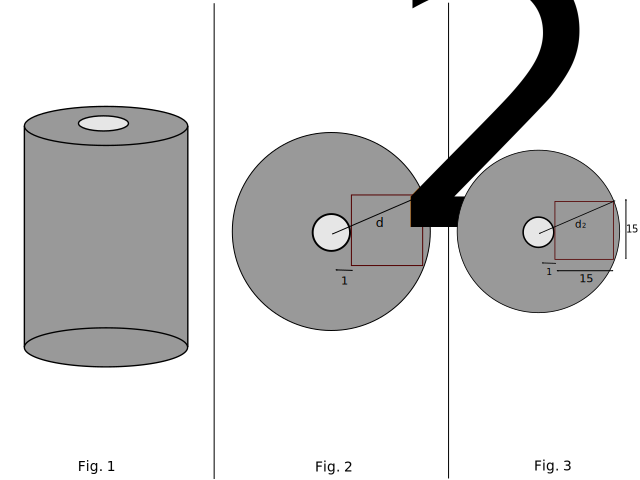
\includegraphics[width=0.75\columnwidth]{img/Q2c.png} % Q2_2nd Image
\end{center}
}
\vspace{20pt}
Diagram of Manipulator Reach

From the problem statement, we have $d_3 \geq 0$ and $1 \leq d_2 \leq d_{2_{max}}$.\\
Also from given problem statement, our work area will take the form of a cylinder with a `hole' in its center, as shown in Fig. 1\\
We need to allow the manipulator to traverse a cube of dimensions $15\times15\times15$, which must fit into the cylinder work area depicted. This is shown is Fig. 2 and Fig. 3.\\

From these figures, we obtain:
\begin{align}
(1+15)^2 + (15/2)^2 = (d_2)^2\\
\implies d_2 = 17.6
\end{align}
This gives us the lower limit for $d_{2_{max}} = 17.6$.\\
Now, $d_3$ must be a minimum of $15$ units, since the the cube has a depth of $15$ units.\\
Lastly, $d_1$ should be a minimum of $15$ units so that joint 3 does not hit the base of the reachable area and allow it unrestricted movement.

Thus, \uuline{$d_1$ must be a minimum of 15 units and $d_{2_{max}}$ must be at least $17.6$ units}.
\end{homeworkSection}
\end{homeworkProblem}

%----------------------------------------------------------------------------------------
%	PROBLEM 3
%----------------------------------------------------------------------------------------

\begin{homeworkProblem}
\problemAnswer{ % Answer
\begin{center}
\includegraphics[width=\columnwidth]{img/Q3_Blocks.png} % Q3_1st Image
\end{center}
}
\vspace{20pt}
SimMechanics Blocks Arrangement

\problemAnswer{ % Answer
\begin{center}
\includegraphics[width=\columnwidth]{img/Q3_Scope.png} % Q3_2nd Image
\end{center}
}
\vspace{20pt}
SimMechanics Scope Output

\problemAnswer{ % Answer
\begin{center}
\includegraphics[width=\columnwidth]{img/Pendulum2.png} % Q3_3rd Image
\end{center}
}
\vspace{20pt}
CAD Model 1

\problemAnswer{ % Answer
\begin{center}
\includegraphics[width=\columnwidth]{img/Pendulum3.png} % Q3_4th Image
\end{center}
}
\vspace{20pt}
CAD Model 2
\end{homeworkProblem}
\clearpage

%----------------------------------------------------------------------------------------
%	PROBLEM 4
%----------------------------------------------------------------------------------------

\begin{homeworkProblem}
\begin{homeworkSection}{(a)}
It is given in problem statement that 
\begin{align}
J=
\begin{bmatrix}
-s_1(a_2c_2 + a_3c_{23}) & -c_1(a_2s_2 + a_3s_{23}) & -a_3c_1s_{23}\\
c_1(a_2c_2 + a_3c_{23}) & -s_1(a_2s_2 + a_3s_{23}) & -a_3s_1s_{23}\\
0 & (a_2c_2 + a_3c_{23}) & a_3c_{23}\\
0 & s_1 & s_1\\
0 & -c_1 & -c_1\\
1 & 0 & 0\\
\end{bmatrix}
\end{align}
Since precise manipulation is required, we need to find the best configuration of angles. To do so, we calculate manipulability $\mu$.\\

For the first configuration given as $\theta_1 = \theta_2 = \theta_3 = 45 \degree$, we have $a = 0.4m$.\\
By calculating $JJ^T$, we obtain 3 non-zero eigenvalues as
\begin{align}
\lambda_1 = 2.64\\
\lambda_2 = 1.08\\
\lambda_1 = 0.06
\end{align}
Now we know that $J$ is a $6 \times 3$ matrix, which gives us a maximum rank of $3$ for the same.
\begin{align}
\mu_1 = K \times |\sqrt{\lambda_1 \lambda_2 \lambda_3}|\\
= 0.43K
\end{align}

For the second configuration given as $\theta_1 = 45 \degree, \theta_2 = -45 \degree, \theta_3 = 45 \degree$, we have $a = 0.4m$.\\
By calculating $JJ^T$, we obtain 3 non-zero eigenvalues as
\begin{align}
\lambda_1 = 2.64\\
\lambda_2 = 1.46\\
\lambda_1 = 0.06
\end{align}
Now we know that $J$ is a $6 \times 3$ matrix, which gives us a maximum rank of $3$ for the same.
\begin{align}
\mu_2 = K \times |\sqrt{\lambda_1 \lambda_2 \lambda_3}|\\
= 0.503K
\end{align}

For the third configuration given as $\theta_1 = 30 \degree, \theta_2 = -30 \degree, \theta_3 = 30 \degree$, we have $a = 0.4m$.\\
By calculating $JJ^T$, we obtain 3 non-zero eigenvalues as
\begin{align}
\lambda_1 = 2.69\\
\lambda_2 = 1.55\\
\lambda_1 = 0.06
\end{align}
Now we know that $J$ is a $6 \times 3$ matrix, which gives us a maximum rank of $3$ for the same.
\begin{align}
\mu_3 = K \times |\sqrt{\lambda_1 \lambda_2 \lambda_3}|\\
= 0.509K
\end{align}
From the values of $\mu_1, \mu_2, \mu_3$, we see that $\mu_3$ has the highest manipulability value.\\
Thus for the configuration given as $\theta_1 = 30 \degree, \theta_2 = -30 \degree, \theta_3 = 30 \degree$, we have the best choice of joint angles for the best manipulability.
\end{homeworkSection}

\begin{homeworkSection}{(b)}
We have, from the problem statement,
\begin{align}
F = 
\begin{bmatrix}
1 & 1 & 1 & 1 & 1 & 1
\end{bmatrix}
\end{align}
where $\theta_1 = 30 \degree$, $\theta_2 = -30 \degree$, $\theta_3 = 30 \degree$\\
We find the torque $\tau$ (calculated in MATLAB) as
\begin{align}
\tau = J^{T} \times F\\
= \begin{bmatrix}
1.2732\\
0.6536\\
0.034
\end{bmatrix}
\end{align}
\end{homeworkSection}
\end{homeworkProblem}
\clearpage

%----------------------------------------------------------------------------------------
%	PROBLEM 5
%----------------------------------------------------------------------------------------

\begin{homeworkProblem}
\begin{homeworkSection}{(a)}
Initial conditions for the system is given as $x_1 = x_2 = x_3 =  0$. Also, the length of the springs at rest is also $0$.\\
This implies that all the blocks at $t=0$ are at same position. As we apply force $F(t)$, the mass $M_1$ starts moving. Since $M_2$ is connected to $M_1$ via the spring-damper system, and similarly since $M_3$ is connected to $M_2$ by the second spring-damper system, the motion of $M_1$ causes all three masses to move.\\
From this explanation, we have the following set of equations:
\begin{align}
M_1\ddot x = F(t) - k_1(x_1 - x_2) - B_1(\dot x_1 - \dot x_2)\\
M_2\ddot x = k_1(x_1 - x_2) + B_1(\dot x_1 - \dot x_2) - k_2(x_2 - x_3) - B_2(\dot x_2 - \dot x_3)\\
M_3\ddot x = k_2(x_2 - x_3) - B_2(\dot x_2 - \dot x_3) - k_3(x_3) - B_3 \dot x_3
\end{align}
\end{homeworkSection}
\begin{homeworkSection}{(b)}
\problemAnswer{ % Answer
\begin{center}
\includegraphics[width=\columnwidth]{img/Simcape.png}
\end{center}
}
\vspace{20pt}
Simscape Diagram

\problemAnswer{ % Answer
\begin{center}
\includegraphics[width=\columnwidth]{img/SimscapeScope.PNG}
\end{center}
}
\vspace{20pt}
Simscape Scope Output
\end{homeworkSection}
\end{homeworkProblem}
\clearpage

\end{document}